\documentclass[11pt]{exam} 
\usepackage{tkz-euclide}
\begin{document} 
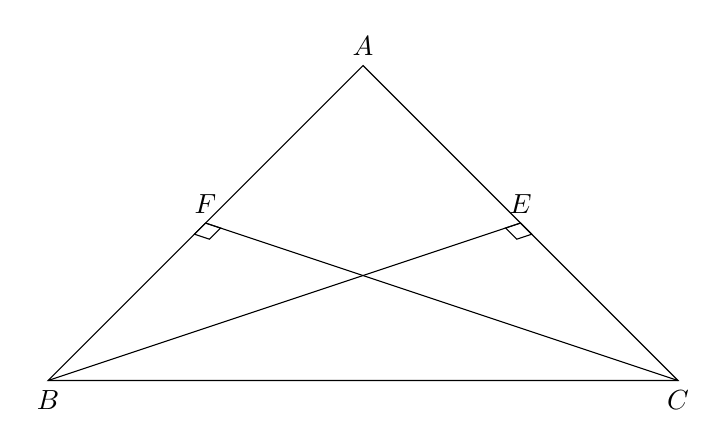
\begin{tikzpicture} 
        \coordinate (A) at (4, 4) {};
        \coordinate (B) at (0, 0) {};
        \coordinate (C) at (8, 0) {};
        \coordinate (E) at (6, 2) {};
        \coordinate (F) at (2, 2) {};
        \draw (A)node[above]{$A$}--(B)node[below]{$B$}--(C)node[below]{$C$}--cycle;
\draw (B)node[below]{}--(E)node[above]{$E$};
\draw (C)node[below]{}--(F)node[above]{$F$};
\tkzMarkRightAngle[size=.2](B,E,C);
\tkzLabelAngle[dist=.5](B,E,C){};
\tkzMarkRightAngle[size=.2](C,F,B);
\tkzLabelAngle[dist=.5](C,F,B){};
\end{tikzpicture}
\end{document}